% fig01 — deployment topology, TikZ remake of the hand-drawn fabric_topology6.
% Fixes audit L6: org naming is now uniform ("Regulator" / "LawFirmA" /
% "LawFirmB" in orderer parentheses, "Org: <name>" as peer-box headers), and
% CID is expanded in-figure. Compile:  tectonic topology.tex  -> topology.pdf,
% then ship as figures/fabric_topology6.pdf.
\documentclass[tikz,border=6pt]{standalone}
\renewcommand{\familydefault}{\sfdefault}
\usetikzlibrary{positioning,arrows.meta,fit,calc,backgrounds}
\pgfdeclarelayer{deep}\pgfdeclarelayer{mid}\pgfsetlayers{deep,mid,main}
\definecolor{navy}{HTML}{1D3C63}
\definecolor{midblue}{HTML}{4478B0}
\definecolor{paleblue}{HTML}{C2D5E9}
\definecolor{bandblue}{HTML}{E4EAF1}
\definecolor{edgecol}{HTML}{1A1A1A}

\begin{document}
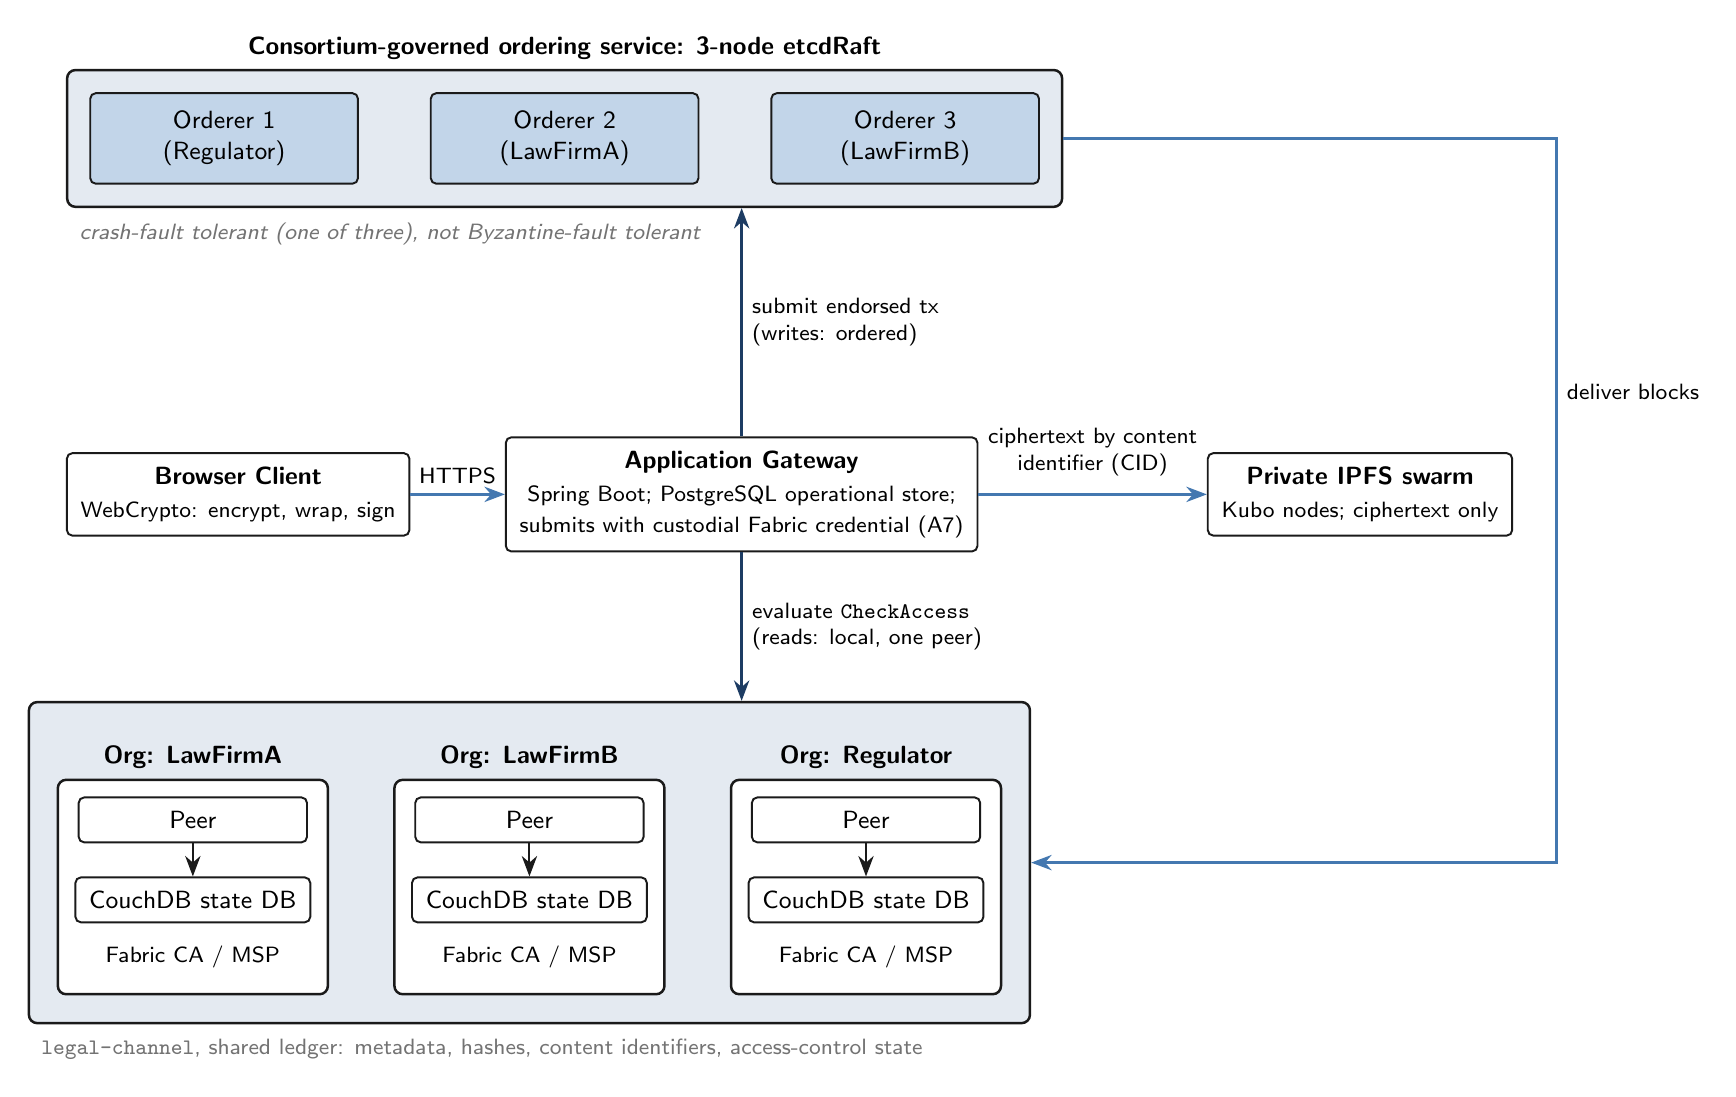
\begin{tikzpicture}[
  font=\small,
  box/.style={draw=edgecol, line width=0.7pt, rounded corners=2pt,
              fill=white, align=center, inner sep=5pt},
  hdrbox/.style={box, fill=paleblue},
  container/.style={draw=edgecol, line width=0.9pt, rounded corners=3pt,
                    fill=bandblue, inner sep=8pt},
  lbl/.style={align=center, text=edgecol},
  note/.style={align=left, font=\footnotesize\itshape, text=black!55},
  arr/.style={-{Stealth[length=2.6mm]}, line width=0.9pt, draw=midblue},
  darr/.style={arr, draw=navy},
]

% ─── ordering service (top) ────────────────────────────────────────────────
\node[hdrbox, minimum width=3.4cm, minimum height=1.15cm] (ord1)
  {Orderer 1\\(Regulator)};
\node[hdrbox, minimum width=3.4cm, minimum height=1.15cm, right=0.9cm of ord1] (ord2)
  {Orderer 2\\(LawFirmA)};
\node[hdrbox, minimum width=3.4cm, minimum height=1.15cm, right=0.9cm of ord2] (ord3)
  {Orderer 3\\(LawFirmB)};
\begin{pgfonlayer}{deep}
\node[container, fit=(ord1)(ord2)(ord3),
      label={[font=\small\bfseries]above:{Consortium-governed ordering service: 3-node etcdRaft}}]
  (ordbox) {};
\end{pgfonlayer}
\node[note, anchor=north west] at ($(ordbox.south west)+(0.05,-0.06)$)
  {crash-fault tolerant (one of three), not Byzantine-fault tolerant};

% ─── middle row ────────────────────────────────────────────────────────────
\node[box, minimum width=3.5cm, below=2.6cm of ordbox.south west, anchor=north west, yshift=-0.5cm]
  (browser) {\textbf{Browser Client}\\[1pt]
             {\footnotesize WebCrypto: encrypt, wrap, sign}};
\node[box, minimum width=5.2cm, right=1.2cm of browser] (gw)
  {\textbf{Application Gateway}\\[1pt]
   {\footnotesize Spring Boot; PostgreSQL operational store;}\\
   {\footnotesize submits with custodial Fabric credential (A7)}};
\node[box, minimum width=3.6cm, right=2.9cm of gw] (ipfs)
  {\textbf{Private IPFS swarm}\\[1pt]
   {\footnotesize Kubo nodes; ciphertext only}};

\draw[arr] (browser) -- node[above, font=\footnotesize]{HTTPS} (gw);
\draw[arr] (gw) -- node[above=3pt, font=\footnotesize, align=center]
  {ciphertext by content\\identifier (CID)} (ipfs);
\draw[darr] (gw.north) -- node[right, font=\footnotesize, align=left]
  {submit endorsed tx\\(writes: ordered)} (gw.north |- ordbox.south);

% ─── peers (bottom) ────────────────────────────────────────────────────────
\newcommand{\orgstack}[3]{%
  \node[box, minimum width=2.9cm, #2] (#1peer) {Peer};
  \node[box, minimum width=2.9cm, below=0.42cm of #1peer] (#1couch) {CouchDB state DB};
  \draw[arr, draw=edgecol, line width=0.7pt] (#1peer) -- (#1couch);
  \node[below=0.16cm of #1couch, font=\footnotesize] (#1ca) {Fabric CA / MSP};
  \begin{pgfonlayer}{mid}
  \node[container, fill=white, inner sep=6pt, fit=(#1peer)(#1couch)(#1ca),
        label={[font=\small\bfseries]above:{Org: #3}}] (#1org) {};
  \end{pgfonlayer}
}
\orgstack{a}{below=2.6cm of browser.south west, anchor=north west, xshift=0.15cm, yshift=-0.7cm}{LawFirmA}
\orgstack{b}{right=1.35cm of apeer}{LawFirmB}
\orgstack{r}{right=1.35cm of bpeer}{Regulator}

\coordinate (hdrpad) at ($(aorg.north)+(0,0.62)$);
\begin{pgfonlayer}{deep}
\node[container, fit=(aorg)(borg)(rorg)(hdrpad), inner sep=10pt] (peersbox) {};
\end{pgfonlayer}
\node[note, anchor=north west, font=\footnotesize]
  at ($(peersbox.south west)+(0.05,-0.06)$)
  {\texttt{legal-channel}, shared ledger: metadata, hashes, content identifiers, access-control state};

\draw[darr] (gw.south) -- node[right, font=\footnotesize, align=left]
  {evaluate \texttt{CheckAccess}\\(reads: local, one peer)} (gw.south |- peersbox.north);

% ─── deliver blocks (right side) ───────────────────────────────────────────
\coordinate (rail) at ($(ipfs.east)+(0.55,0)$);
\draw[arr] (ordbox.east) -- (ordbox.east -| rail)
  -- node[right, font=\footnotesize, pos=0.35]{deliver blocks}
  (peersbox.east -| rail) -- (peersbox.east);

\end{tikzpicture}
\end{document}
